%%=====================================================================================================
%%
%% AERMET:
%%-----------------------------------------------------------------------------------------------------
%\subtitle{AERMET: Fundamentos}
% \begin{frame}{}
%     \maketitle
% \end{frame}
% 
% \begin{frame}{AERMET}{Pre-procesador meteorológico del AERMOD}
%Usa mediciones meteorologicas y computa parámetros de la capa límite que permiten a AERMOD estimar perfiles de vientos, turbulencia y temperatura.
%Los parámetros calculados por AERMET son:
%\begin{itemize}
%\item Flujo de Calor ($H$)
%\item Velocidad de fricción ($ u* $)
%\item Longitud de Monin-Obukhov ($L$)
%\item Escala de velocidad convectiva ($ w* $)
%\end{itemize}
%
%%El crecimiento y estructura de la CLP está regulada por los flujos de calor y momentum que a su vez dependen de efectos de la superficie. El espesor de esta capa está incluenciada a escala local por características de la superficie: rugosidad ($z0$), albedo ($a0$), y disponibilidad de humedad ($b0$).
%
%Además estima alturas de mezcla mecánica ($z_{im}$) y convectiva ($z_{ic}>$). Y define la estabilidad de la CLP por el signo de $H$ (convectiva si H>0 y estable si H<0).
%%
%\end{frame}
%
%\begin{frame}{AERMET}{Archivos de salida}
%
%El AERMET genera dos archivos de salida:
%
%
%\begin{columns}[t]
%\column{0.5\textwidth}
%\texttt{*.SFC}
%\begin{table}
%\small
%\centering
%\begin{tabular}{c| l}
%1-5             & fecha y hora \\
%6               & H (W/m 2) \\
%7               & $u_*$ (m/s) \\
%8               & $w_*$ (m/s) \\
%9               & $d\theta/dz$ (K/m) \\
%10              & $z_{ic}$ (m) \\
%11              & $z_{im}$ (m) \\
%12              & $L$ Monin-Obukhov (m)\\
%13-15           & $z_0$, $b_0$, $a_0$\\
%    16-27           & datos usados (u,T,ppt,p,etc.)\\
%%16-18           & $u$ \\
%%19-20           & $T$ \\
%%21-22           & precipitación \\
%%23              & humedad relativa \\
%%24              & presión \\
%%25              & cobertura de nubes \\
%%26              & $u$ ajustado \\
%%27              & flag interpolacion \\
%\end{tabular}
%\end{table}
%
%\column{0.5\textwidth}
%    
%\texttt{*.PFL}
%\begin{table}
%\small
%\centering
%\begin{tabular}{c| l}
%1-4         &  fecha y hora  \\
%5           &  altura de medicion (m)  \\
%6           &  indicador: 1/0 (ultimo nivel)\\
%7-8         &  direccion y velocidad de viento \\
%9           &  temperatura \\
%10          &  $\sigma_\theta$ - desvio de dirección del viento\\
%11          &  $\sigma_w$ desvio de velocidad del viento
%    \end{tabular}
%\end{table}
%\end{columns}
%    
%\end{frame}
%
%
%
% 
%\begin{frame}{Balance de energía}{Cálculo de calor sensible \footnote{$R_n$: radiación neta. $H$: calor sensible. $\lambda E$: calor latente. $G$: flujo de calor al suelo.}}
% 
%\begin{center}
%\begin{tikzpicture}[scale=0.5]
%    \begin{scope}
%    \piso{-3}{3}{0}
%    \draw[-latex,very thick] (-2.5, 2.0) -- (-2.0, 0.0) node[midway,anchor=east]{$\mathrm{R_n}$} ;
%    \draw[-latex,very thick] (-1.0, 0.0) -- (-0.5, 2.0) node[midway,anchor=west]{$\lambda \mathrm{E}$  };
%    \draw[-latex,very thick] ( 0.0, 0.0) -- ( 0.0,-1.0) node[midway,anchor=west]{$\mathrm{G}$  };
%    \draw[-latex,very thick] ( 1.0, 0.0) -- ( 1.5, 2.0) node[midway,anchor=west]{$\mathrm{H}$  };
%    \end{scope}
%\end{tikzpicture}
%\end{center}
%\vspace{-0.5em}
%$$ R_n = H + \lambda E + G$$
% 
%Considerando:\footnote{$B_0$: Relación de Bowen, depende del tipo de cobertura.}
%$$ G \approx 0.1 R_n \qquad B_0 =\dfrac{\lambda E}{H}  $$
% 
%El calor sensible (H) se puede calcular como:
%$$ 
%H = \dfrac{0.9\,R_n}{ 1 + 1/B_0}
%\qquad
%\begin{cases}
%    H<0  & \text{Flujo atmosfera a superifice (ESTABLE)}  \\
%    H=0  & \text{No hay flujo neto (NEUTRO)}  \\
%    H>0  & \text{Flujo superficie a atmosfera (INESTABLE)}
%\end{cases}
%$$
%\end{frame}
% 
%\begin{frame}{Balance Radiativo}{Radiación Neta}
% 
%\begin{center}
%\begin{tikzpicture}[scale=0.9]
%    \begin{scope}
%    \piso{-3}{3}{0}
%    \draw[-latex,very thick] (-2.5, 2.0) -- (-2.0, 0.1) node[midway,anchor=east]{\small$\mathrm{R}$} ;
%    \draw[-latex,very thick] (-1.8, 0.1) -- (-1.3, 2.0) node[midway,anchor=west]{\small$rR$};
%    \draw[-latex,very thick] (-0.5, 2.0) -- (-0.5, 0.1) node[midway,anchor=west]{\small$c_1T^6$};
%    \draw[-latex,very thick] ( 1.0, 0.1) -- ( 1.0, 2.0) node[midway,anchor=west]{\small$\sigma T^4$};
%    \draw[-latex,very thick] ( 2.5, 1.5) -- ( 2.5, 0.2) node[midway,anchor=west]{\small$c_2\,n$};
%    
%    \draw[scale=0.4,xshift=7cm, yshift=4cm] (-1.6,-0.7) .. controls (-2.3,-1.1) and (-2.7,0.3) .. (-1.7,0.3) .. controls (-1.6,0.7)and (-1.2,0.9) .. (-0.8,0.7) .. controls (-0.5,1.5) and (0.6,1.3) .. (0.7,0.5) .. controls (1.5,0.4) and (1.2,-1) .. (0.4,-0.6) .. controls (0.2,-1) and (-0.2,-1) .. (-0.5,-0.7) .. controls (-0.9,-1) and (-1.3,-1) .. cycle;
% 
%    \end{scope}
%\end{tikzpicture}
%\end{center}
% 
%$$ R_n = \dfrac{R - r\,R + c_1 T^6 + c_2 \,n - \sigma T^4}{1 + c_3} $$
% 
% 
% 
%donde:
%\begin{itemize}
%    \item $R - rR    $ : Radiación incidente menos albedo.
%    \item $c_1 T^6   $ : Absorción de GEIs.
%    \item $\sigma T^4$ : Emisión de superficie (Stephan-Boltzman).
%    \item $c_2 \, n  $ : Emisión de las nubes.
%\end{itemize}
% 
%\end{frame}
% 
% 
%\begin{frame}{Balance Radiativo}{Radiación incidente}
%  
%\begin{center}
%\begin{tikzpicture}[scale=0.9]
%    
%    \draw[fill=black!10,scale=0.4,xshift=0cm, yshift=3cm] (-1.6,-0.7) .. controls (-2.3,-1.1) and (-2.7,0.3) .. (-1.7,0.3) .. controls (-1.6,0.7)and (-1.2,0.9) .. (-0.8,0.7) .. controls (-0.5,1.5) and (0.6,1.3) .. (0.7,0.5) .. controls (1.5,0.4) and (1.2,-1) .. (0.4,-0.6) .. controls (0.2,-1) and (-0.2,-1) .. (-0.5,-0.7) .. controls (-0.9,-1) and (-1.3,-1) .. cycle;
%    \piso{-2}{1}{0}
%    \draw[-latex,very thick] (-1.5, 2.0)--(0.0, 0.0) node[midway,anchor=east]{$\mathrm{R}$} ;
%    
%    \coordinate (O) at (0,0);
%    \coordinate (A) at (-1,0) ;
%    \coordinate (B) at (-1.5,2);
%    \pic[draw,black,  angle eccentricity=1.5]{angle=B--O--A} node[anchor=south east,xshift=-10pt] {$\phi$};
%    
%    %sol:
%   \fill[yellow!30](-1.7,2.2) circle[radius=.25cm];
%   \fill[orange!60](-1.7,2.2) circle[radius=.2cm];
% 
%\end{tikzpicture}
%\end{center}
% 
%Holtslag y Ulden (1983):\footnote{donde Ángulo de Elevación Solar: $\phi=\arcsin (sin\lambda \sin\delta + \cos\lambda\cos\delta\cosh)$, con $\lambda$:latitud, $\delta$: declinación, y h el ángulo horario. Fracción nubosa: $n$.}
%$$  R = (990 \sin(\phi) - 30 ) \, (1-0.75 n^{3.4}) $$
% 
%\end{frame}
% 
% 
%
%\begin{frame}{Caracterización de CLP}{Similitud}
%    
%\end{frame}
%
%
%\begin{frame}{Caracterización de CLP}{Velocidad de fricción}
%    
%    
%    $$
%    u_*=\sqrt{\dfrac{\tau}{\rho}}
%    $$
%    
%
%\end{frame}
%
%\begin{frame}{Caracterización de CLP}{Longitud de Monin-Obukhov}
%
%    Representa la altura (en metros) sobre la cual la produccion mecánica de turbulenta es alanceada con la producción de empuje térmico.
%    $$
%        L=\dfrac{-\rho \,c_p\,T_a\,u_*^3 }{g\,\kappa\,H}
%    $$
% 
%    \begin{itemize}
%        \item Estable: $L > 0$ %(since H < 0) very stable: 0 < L < 10
%        \item Inestable: $L < 0$ %(since H > 0) 
%        %very unstable: -10 < L < 0
%        \item Neutra $|L| > 1000$
%    \end{itemize}
%    
%\end{frame}
%
%\begin{frame}{Caracterización de CLP}{Velocidad convectiva}
%    Related to the vertical velocities in the large
%thermals (i.e., convective eddies)
%Depende de:
%\begin{itemize}
%    \item Magnitude of buoyant turbulent energy
%    \item Scaling height for the eddies (i.e., z i )
%\end{itemize}
% 
% 
%$$
%w_*=\bigg( \dfrac{g\,z_i\,H}{c_p\,\rho\,\theta}\bigg)^{1/3}
%$$
%Valores en el orden de 1-2 metros/segundo
%
%\end{frame}
%
%
%\begin{frame}{Caracterización de CLP}{Perfiles}
%    AERMOD usa relaciones de similitud y observaciones meteorológicas para construir perfiles de viento, temperatura y turbulencia, hasta los 4000 metros en cada hora modelada.
%    
%    
%\end{frame}
%
%\begin{frame}{Caracterización de CLP}{Variables effectivas}
%    
%\end{frame}
%
%%$$
%%
%%Nos queda como incognita la radiación neta R<sub>n</sub> que puede ser observada o estimada.
%%
%%La radiación incidente para cielos claros (R0) está dado por:
%%
%%$$ R_0 = a_1 \sin \phi + a_2 $$
%%
%%Podemos llegar a:
%%
%%$$ R_n = \dfrac{(1- r_{(\phi)}) R + c_1 T^6_{\text{ref}} - \sigma_{SB}T^4_{\text{ref}} - c^2\,n }{1 + c_3} $$
%%
%%
%%
%%\begin{frame}{Estimaciones para atmósfera convectiva}{Balance radiativo}
%%    
%%\end{frame}
%%#### Velocidad de fricción y Longitud de Monin-Obukhov
%%
%%Una vez que se estima el flujo de calor (H), AERMET estima la $u^*$, $L$ mediante un método iterativo, usando las siguentes expresiones:
%%
%%
%%$$
%%u_* = \dfrac{\kappa \,u}{  \ln(z_{\text{ref}}/z0) - \Psi_m(z_{\text{ref}}/L) + \Psi_m(z_{\text{0}}/L)  }
%%$$
%%
%%y 
%%
%%$$ L =-\dfrac{\rho c_p T u_*^3}{\kappa g H} $$
%%
%%
%%
%%$$ \Psi_m (z_0/L) = 2\ln(\dfrac{1+\mu_0}{2})+\ln(\dfrac{1+\mu_0^2}{2}) - 2\tan^{-1}(\mu_0) + 0.5\,\phi $$
%%
%%
%%$$ \Psi_m (z_0/L) = 2\ln(\dfrac{1+\mu_0}{2})+\ln(\dfrac{1+\mu_0^2}{2}) - 2\tan^{-1}(\mu_0) + 0.5\,\phi $$
%%
%%
%%donde 
%%<center>
%%&mu;<sub></sub> = (1 -16 z<sub>ref</sub> / L )<sup>1/4</sup>
%%
%%&mu;<sub>0</sub> = (1 -16 z<sub>0</sub> / L )<sup>1/4</sup>
%%</center>
%%
%%El proceso requere un $u_*$ inicial, que se calcula contemplando los $\Psi$ igual a cero, y luego la iteración continua hasta que los valores de L difieren en menos del 1%.
%%
%%
%%
%%\begin{frame}{Estimaciones para atmósfera convectiva}{Altura de mezcla}
%%    
%%\end{frame}
%%#### Alturas de mezcla:
%%
%%
%%$$
%%z_{ic} \theta(z_{ic}) - \int_0^{z_{ic}} \theta(z) \,dz = (1 + 2A) \int_0^t \dfrac{H(t')}{\rho c_p} dt
%%$$
%%
%%donde &theta;<sub>0</sub>(z) es la distribución vertical de la temperatura potencial dado por el sondeo de la mañana y el término derecho representa el flujo de calor acumulado en z=0. A=0.2
%%
%%Una vez que conocemos z<sub>ic</sub> podemos obtener $w_*$ como:
%%
%%$$
%%w_* = (\dfrac{gHz_{ic}}{\rho c_p T})^{1/3}
%%$$
%%
%%
%
%
%%### Estimación para atmosfera estable
%%\begin{frame}{Estimaciones para atmósfera estable}{Balance radiativo}
%%    
%%\end{frame}
%%Para el caso de atmosferas estables los calculos son más simples y no requieren procesos iterativos
%%
%%
%%
%%Usando
%%<center>
%%H=-D c<sub>p</sub> u<sub>*</sub> &theta;<sub>*</sub>
%%</center>
%%
%%Luego:
%%
%%$$ \kappa \dfrac{u}{u_*} = \ln( \dfrac{z_{\text{ref}}}{z0} ) + \beta_m \dfrac{z_{\text{ref}}}{L}  $$
%%
%%
%%\begin{frame}{Estimaciones para atmósfera estable}{Velocidad de fricción}
%%    
%%\end{frame}
%
%
%%La velocidad de fricción se calcula como:
%%
%%$$ u_* = C_D u/2 (1 + \sqrt{1- (2u_0/\sqrt{C_D} u)^2} ) $$
%%
%%donde 
%%
%%$$ C_D \dfrac{\kappa}{\ln{z_{\text{ref}}/z_0}} $$
%%
%%y 
%%
%%$$ u_0 = \sqrt{\beta_m z_{\text{ref}} g \theta_* / T} $$
%%
%%
%%$$ \theta_* = 0.09 (1-0.5n^2) $$
%%
%%donde $n$ es la fracción opaca por cobertura nubosa.
%%
%%El flujo de calor se computa como :
%%
%%$$H=-\rho c_p u_* \theta_* $$
%%
%%con $ u_* = \hat{u}_* u / \hat{u}_* $ y $ \theta_* =\hat{theta}_* u / \hat{theta}_*$
%%
%%y 
%%
%%$$ z_{im} = 2300 u_*^{3/2} $$
%%
%
%
%
%
%
%
%
%
%\begin{frame}{Turbulencia}{Similitud}
%Variables utilziadas en analisis dimensional: ($\sigma_u$,$u_*$,$L$,$h_{\text{mix}}$, $z$). 
%
%En \alert{condiciones neutras}
%$$
%\sigma_u = u_* 2.5 \,e^{-1.5 \frac{z}{h_{\text{mix}}}}   \bigg)^a
%\qquad
%\sigma_v = u_* 1.6 \bigg(  1- \dfrac{z}{h_{\text{mix}}}  \bigg)^a
%\qquad
%\sigma_w = u_* 1.25 \bigg(  1- \dfrac{z}{h_{\text{mix}}} \bigg)^a
%$$
%
%En condiciones \alert{estables},
%$$
%\sigma_u = u_* 2.2   \bigg(  1- \dfrac{z}{h_{\text{mix}}}   \bigg)^a
%\qquad
%\sigma_v = u_* 2.2 \bigg(  1- \dfrac{z}{h_{\text{mix}}}   \bigg)^a
%\qquad
%\sigma_w = u_* 1.73 \bigg(  1- \dfrac{z}{h_{\text{mix}}}   \bigg)^a
%$$
%\end{frame}
%
%\begin{frame}{Turbulencia}{Similitud}
%En \alert{condiciones inestables}, se define una nueva velocidad de escala convectiva ($w_*$) para contemplar la turbulencia inducida termicamente:
%
%$$ w_* = \bigg( \dfrac{g\,z_i\,H}{c_p\,\rho\,\theta} \bigg) \quad\Rightarrow\quad w_* = \bigg( \dfrac{h_{\text{mix}}}{L\,\kappa}\bigg)^{1/3} $$
%
%Por debajo de la capa de mezcla se obtiene experimentalmente:
%
%$$
%\dfrac{\sigma_u}{w_*}=\dfrac{\sigma_u}{w_*}=\dfrac{\sigma_u}{w_*}=0.6
%$$
% Independientemente de la altura. Por encima de la capa de mezcla la turbulencia decae exponencialmente.
%\end{frame}
%
%
%
%
%\begin{frame}{Altura de capa de mezcla}
% 
%Considerando el mezclado \alert{turbulento mecánico}:
%    $$
%   \text{En condiciones neutrales:}\qquad  h_{\text{mix}}=\dfrac{0.3 u_*}{|f|}
%    $$
%    $$\text{En condiciones estables:}\qquad
%    h_{\text{mix}}=C\sqrt{\dfrac{ u_* L}{|f|}  }
%    $$
%    
%Bajo condiciones inestables, la $h_{\text{mix}}$ esta principalmente determinada por \alert{mezclado térmico}:
%    $$\text{En condiciones inestables:}\qquad
%    h_{\text{mix}}\approx D\sqrt{\dfrac{ u^3_*}{|f|^3L}  }
%    $$
% 
%\end{frame}
%
%
%
%
%=====================================================================================================
%
% AERMOD:
%-----------------------------------------------------------------------------------------------------
\subtitle{AERMOD: Fundamentos}
 \begin{frame}{}
     \maketitle
 \end{frame}
 
\begin{frame}{AERMOD}{Sistema de modelado}
 
 \begin{center}
 \begin{tikzpicture}[
    programa/.style={draw, minimum width=2cm, minimum height=1.2cm },
    archivo/.style={draw, minimum height=3.7em, minimum width=3em, fill=white, copy shadow={shadow xshift=2pt, shadow yshift=2pt, black!30, draw}},]

\begin{scope}[scale=0.3]
       
    %ARCHIVOS:
   \node[archivo,              , align=center] (dem) {MDE\\\texttt{.tiff}};
   \node[archivo, below= 0.2cm of dem, align=center ] (ish) {\texttt{.sam}\\\texttt{.ish}};
   \node[archivo, below= 0.2cm of ish, align=center ] (fsl) {\texttt{.fsl}};
   \node[archivo, below= 0.2cm of fsl, align=center] (lu)  {LU\\\texttt{.tiff}};
   
    %PROGRAMAS:
   \node[programa, right = 3cm of ish          ] (aermet) {AERMET};
   \node[programa, right = 2cm of aermet, fill=blue!10] (aermod) {\textbf{AERMOD}};
   \node[programa, above = 0.5cm of aermet,fill=yellow!20] (aermap) {AERMAP};
   \node[programa, right = 2.65cm of lu        ](aersurface) {AERSURFACE};
   \node[programa, below = 2.3 cm of aermod,fill=yellow!20](bpip) {BPIPPRM};
   
   %variables:
   \node[red!80, below = -0.5cm of aermet, align=center] {\small $u_*$,$w_*$,$H$,$L$\\\small$d\theta/dz$,$z_{ic}$,$z_{im}$\\\small $\sigma_w$, $\sigma_\theta$};
   \node[red!80, below = -0.5cm of aersurface] {\small $a_0$,$b_0$,$z_0$};
   \node[red!80, below = -0.5cm of aermap] {\small $z_r$,$z_h$,$z_p$};
   \node[red!80, below = -0.5cm of bpip, align=center] {\small $b_{len}$,$b_{hgt}$,$b_{wid}$\\,$x_{badj}$,$y_{badj}$};
   
   %Flechitas
   \draw[-latex,thick,black!60] (aersurface.north) -- (aermet.south) node[midway,left]{\small\texttt{.out}};
   \draw[-latex,thick,black!60] (ish.east) edge (aermet.west);
   \draw[-latex,thick,black!60] (fsl.east) edge ([yshift=-0.3cm] aermet.west);
   \draw[-latex,thick,black!60] (lu.east) edge (aersurface.west);
   \draw[-latex,thick,black!60] (dem.east) edge (aermap.west);
   \draw[-latex,thick,black!60] (aermap.east) -- ([yshift=3cm] aermod.north)--(aermod.north) node[midway,right]{\small\texttt{.rou}};
   \draw[-latex,thick,black!60] (aermet.east) -- (aermod.west) node[midway,below]{\texttt{.pfl}} node[midway,above]{\texttt{.sfc}};
   \draw[-latex,thick,black!60] (bpip.north) -- (aermod.south) node[midway,right]{\small\texttt{.out}};
\end{scope}
\end{tikzpicture}
\end{center}

\end{frame}


\begin{frame}{AERMOD}{Características generales}
    
    \begin{itemize}
        \item Modelo de pluma gaussiano de estado estacionario.
        \item Usa parametrización continua para los coeficientes de dispersión ($\sigma_{y,\,z}$).
        \item Caracteriza la capa límite, usando la teoria de similitud para representar las variables en el perfil de esta.
        \item Contempla inhomogeneidades de la PBL mediante el uso de \textit{variables efectivas}.
        \item Representa la dispersión en terrenos complejos.
        \item Contempla corrientes ascendentes y descendentes mediante una distribución vertical bi-gaussiana.
        \item Representa \textit{plume lofting} y la inyección de plumas flotantes a capas estables.
    \end{itemize}
\end{frame} 

\section{Interfaz meteorológica}
\begin{frame}{Cálculo de perfiles}{Perfil de viento}

Sigue el típico patron logarítmico:
$$
u(z) = \begin{cases}
    u_(z_i) & z > z_i  \\
     \dfrac{u_*}{\kappa} \bigg[ \ln{\dfrac{z}{z_0}} - \Psi(z/L) + \Psi(z_0/L )\bigg]&  7z_0 < z < z_i\\[0.8em]
    \dfrac{z}{7\,z_0}u_{(7z_0)} & z < 7z0  \\[0.8em]
\end{cases}
$$
Para condiciones \alert{estables}:
$$ 
\Psi(\frac{z}{L}) = 17 \exp\bigg(-0.29\dfrac{z}{L}\bigg)
$$
 
 En condiciones \alert{inestables}:
 $$
 \Psi( \frac{z}{L}) =  2\,\ln \frac{2 - 16\,z/ L}{2} + \ln \frac{1+(1 - 16\,z/L)^2}{2} - 2 \arctan( (1 - 16\,z / L) + \pi/2 )
 $$
   
\end{frame}

%\begin{frame}{Cálculo de perfiles}{Gradiente de temperatura potencial}
%
%Para condiciones \alert{estables} se calcula:
%    $$
%     \dfrac{\partial \theta}{\partial z} (z)=
%     \begin{cases}
%       % \dfrac{\theta_*}{k(2)}\bigg( 1+ 5 \dfrac{2}{L}\bigg) &  z < 2m\\[0.8em]
%        \dfrac{\partial \theta}{\partial z}\bigg\rvert_{100} \exp{ \bigg[ - \dfrac{z-100}{0.44\,z_{i\,\theta}} \bigg] } & z >100m \\[1em]
%        \dfrac{\theta_*}{k\,z}\bigg( 1+ 5 \dfrac{z}{L}\bigg) & 2m < z < 100m  \\[0.8em]
%        \dfrac{\partial \theta}{\partial z} \bigg\rvert_{2}  &  z < 2m\\[0.8em]
%    \end{cases}
%    $$
% Bajo condiciones \alert{inestables} se asume que el gradiente es constante:
% $$\dfrac{\partial \theta}{\partial z} = 0 $$
% \end{frame}
% 
%\begin{frame}{Cálculo de perfiles}{Temperatura potencial}
% 
% Una vez conocido el perfil del gradiente de la temperatura potencial, se puede calcular la temperatura potencial como:
% 
% $$
% \theta(z+\Delta z) = \theta(z) + \dfrac{\partial \theta}{\partial z}\bigg\rvert_{z} \Delta z
% $$
% 
% Para esto es necesario conocer $\theta$ en algun punto de referencia:
% 
% $$
% \theta_{ref} =T_{ref}+\dfrac{g}{c_p}\,z_{mls}
% $$
% 
% donde: 
% $$z_{mls}=z_{ref}+z_{base}$$
%\end{frame}
%
%\begin{frame}{Cálculo de perfiles}{Coeficiente turbulento vertical}
%    
%Se puede separar en una componente convectiva y otra mecánica:
%    $$ 
%    \sigma_w^2 = \sigma_{wc}^2 + \sigma_{wm}^2
%    $$
%    
%    
%    $$
%    \sigma_{w\,c}^2 = 1.6\, w_*^2\, \bigg(\dfrac{z}{z_i}\bigg)^{2/3} \qquad \sigma_{w\,m}^2 =1.3u_*\sqrt{1-\dfrac{z}{z_i}}
%    $$
%    
%\end{frame}

%\begin{frame}{Cálculo de perfiles}{Coeficiente turbulento vertical}
%    También se puede separar en una componente convectiva y otra mecánica:
% 
%     $$ 
%     \sigma_{v\,c}^2 = \sigma_{vc}^2 + \sigma_{vm}^2
%     $$
%     
%     $$
%     \sigma_{v\,m}^2 = 0.35\,w_*^2 \qquad \sigma_v^2 = 3.6 \, u_*^2
%     $$
%     
%    
%\end{frame}


\begin{frame}{Cálculo de variables efectivas}
 
% Las plumas se extienden en todo el espacio, pero los parámetros de la pluma solo pueden tomar un valor para representar la atmósfera, aunque estas cambien en el espacio. Esto es una fuente de error pero puede reducirse usando valores adecuados promedios para asegurar la representatividad.
 
El proceso de calcular variables efectivas puede resumirse en:
\begin{itemize}
 \item Cálculo de altura del centroide de la pluma ($h_c$) 
 \item Cálculo de $\sigma_z$ en base a los valores de $\sigma_w$ y $h_c$
 \item Se considera el menor de los intervalo entre $h_c$ y el receptor ($z_r$) ó entre $h_c$ y $2.15\sigma_z$ en la dirección del receptor.
 \item La variable de interés es integrada entre el intervalo vertical definido en el paso previo y dividido por el dicho intervalo para obtener la variable efectiva.
\end{itemize}

Por ejemplo, la velocidad efectiva: \footnote{No confundir con la velocidad promedio $\overline{u}=1/z_i \, \int_0^{z_i} u(z) dz$}
    $$\tilde{u} = \dfrac{1}{h_c - z_r} \int_{z_r}^{h_c} u(z) dz $$
    
\end{frame}

    


\section{Cálculo de concentraciones}
 
\begin{frame}[t]{Terreno complejo}{}
 
 AERMOD calcula dos plumas: una ignorando el terreno y otra siguiendo el terreno.
  
\begin{center}
\begin{tikzpicture}[scale=1]
\ejesXZ{-5}{0}{0.45}
\piso{-4}{4.5}{0}
\chimenea{-3.1}{0}{0.2}{1}
%pluma real
\fill[red!20,opacity=0.5] (-3,1) -- (4,2) -- (4,0.4) -- (-3,1);
%mountain
\draw[ latex-latex] (-3.2, 1)--(-3.2,0) node[midway, anchor=east]{$h_s$};
 
     \node[brown] at (0.5,0.8) {\textbullet};
     \fill[fill=blue] (0.5,1.1) circle[radius=2pt] node[left]{$r_1$};
     \fill[fill=red ] (0.5,0.3) circle[radius=2pt] node[left]{$r_2$};
     
     \draw[latex-latex] (0.5,0.8)--(0.5,1.1)node[midway,anchor=west]{$z_{p}$}; 
     \draw[latex-latex] (0.5,0.0)--(0.5,0.3)node[midway,anchor=west]{$z_{p}$}; 
    % \draw[latex-latex] (1.5,0.0)--(1.5,1.1)node[midway,anchor=west]{$z_{r}$};
    % \draw[latex-latex] (1.0,0.0)--(1.0,0.8)node[midway,anchor=west]{$z_{t}$}; 
     
   \draw[orange!70, dashed] (-3,0.85)--(5,0.85) node[anchor=west]{$H_c$};
   \draw[|-|, green] (4.0,0.85)--(4.0,2.0) node[midway, anchor=west]{$M_a$};
   \draw[|-|, green] (4.0,0.85)--(4.0,0.5) node[midway, anchor=west]{$M_b$};
   \draw[clip]
    decorate [decoration={random steps,segment length=3pt,amplitude=1pt}]%
    {(-1,0) --(0,0.3)-- (0.5,0.8) -- (1,1.5)--(2,2) --(3.0,2.5)-- (3.5,2.3) -- (4,0)}-- (0,0) -- (-1,0);
    \fill[rock](-1,0) rectangle (4,4);
        
\end{tikzpicture}
\end{center}
 
 la concentración final es la suma ponderada de estas dos: \footnote{donde $f=0.5 + 0.5 \varphi_p $ y $\varphi_p= M_b / M_a\,M_b$. $M_a$ Masa sobre $H_c$ y $M_b$ masa por debajo de $H_c$. $H_c$: critical dividing streamline, depende de $h_c$: hill slope scale (calculado en AERMAP).}

  $$ C_{tot} = f {\color{blue} C_{ref} } + (1-f) {\color{red}C_{terr.} } $$



\end{frame}
 
 
\begin{frame}{Cálculo de dispersión}{Fórmula general}

    $$
        \overline{c} = \dfrac{Q}{\tilde{u}}\,\varphi_y\,\varphi_z
    $$
    
$\varphi_y$ es la dispersión horizontal:
$$
\varphi_y =\dfrac{1}{\sqrt{2\pi}\sigma_y}\exp{\bigg(-\dfrac{1}{2}\dfrac{y^2}{\sigma_y^2}\bigg)}
$$

la dispersión vertical $\varphi_z$ tambien tiene forma \textit{gaussiana} en \alert{atmósferas estables}:
$$
\varphi_z =\dfrac{1}{\sqrt{2\pi}\sigma_z} \bigg\{ \exp{\bigg[-\dfrac{1}{2}\dfrac{(z+h_c)^2}{\sigma_z^2}\bigg]} + \exp{\bigg[-\dfrac{1}{2}\dfrac{(z-h_c)^2}{\sigma_z^2}\bigg]} \bigg\}
$$

%\footnote{
donde $h_c$ es la altura del centro de la pluma. 
$$h_c=h_s + \Delta z$$
%}
\end{frame}
 
 
 
\begin{frame}{Cálculo de dispersión}{Elevación de la pluma (\textit{plumerise})}
    
    La elevación se calcula usando los flujos de momentum ($F_m$) y empuje ($F_b$)\footnote{ donde $F_m=w_s^2\,r_s^2 T/T_s$ y $F_b=g\,w_s\,r_s^2 \Delta T/T_s$ }
  
  $$ \Delta z = \bigg( \dfrac{3\,F_m\,x}{0.36\,u_{(h_s)}^2} + \dfrac{3\,F_b\,x}{0.72\,u_{(h_s)}^3} \bigg)^{1/3}$$
 \begin{center}
  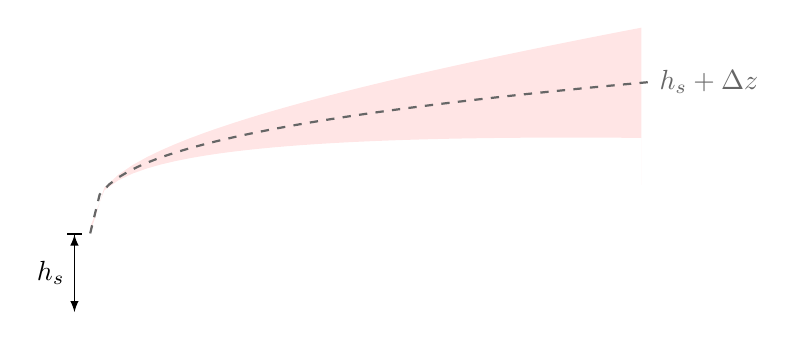
\begin{tikzpicture}
      \ejesXZ{-5}{0}{0.45}
      \piso{-4}{4.5}{0}
      \chimenea{-3.1}{0}{0.2}{1}
       \fill[red!20,opacity=0.5] plot[domain=-3:4,samples=40]({\x},{1+(\x+3)^(1/3)+(\x+3)*0.1})--++(0,-2)--plot[domain=4:-3,samples=40]({\x},{1+(\x+3)^(1/3)-(\x+3)*0.1});
       \draw[thick, black!60,dashed] plot[domain=-3:4.1,samples=60]({\x},{(\x+3)^(1/3)+1}) node[right]{$h_s + \Delta z$};
      \draw[| latex-latex] (-3.2, 1)--(-3.2,0) node[midway, anchor=east]{$h_s$}; 
 \end{tikzpicture}
 \end{center}
    
\end{frame}
 



\begin{frame}{Cálculo de dispersión}{Updrafts y Downdrafts}
 
 Bajo condiciones \alert{inestables} hay corrientes verticales ascendentes y descendentes:
 
 \begin{center}
 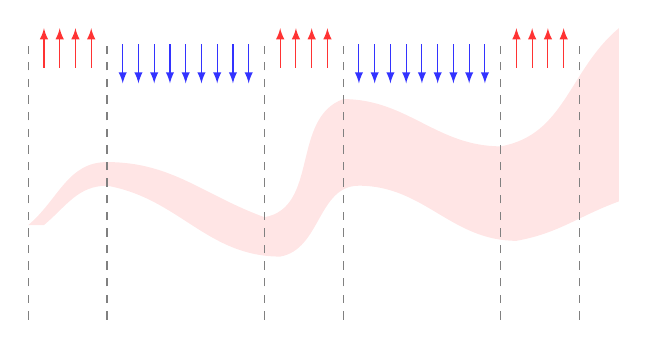
\begin{tikzpicture}[scale=1.0]
 \ejesXZ{-5}{0}{0.45}
 \piso{-4}{4.5}{0}
 \chimenea{-3}{0}{0.2}{1.2}
 %pluma real
 \fill[red!20,opacity=0.5] (-2.8,1.2) to[out=40 ,in=180] 
                           (-2. ,1.7) to[out=-10,in=180]
                           (0.2 ,0.8) to[out=10 ,in=180]
                           (1.2 ,1.7) to[out=  0,in=180]
                           (3.2 ,1.0) to[out=10 ,in=200]
                           (4.5 ,1.5) -- 
                           (4.5 ,3.7) to[out=220 ,in= 10]
                           (3.0 ,2.2) to[out=180 ,in=  0]
                           (1.0 ,2.8) to[out=200 ,in= 10]
                           (0.0 ,1.3) to[out=160 ,in=  0]
                           (-2. ,2.0) to[out=180 ,in= 40] (-3.0,1.2);
 %\draw[ latex-latex] (-3.2, 1.2)--(-3.2,0) node[midway, anchor=east]{$h_s$};
         
 \draw[dashed,black!50] (-3.0, 0.0)--++(0,3.5);
 \draw[dashed,black!50] (-2.0, 0.0)--++(0,3.5);
 \draw[dashed,black!50] ( 0.0, 0.0)--++(0,3.5);
 \draw[dashed,black!50] ( 1.0, 0.0)--++(0,3.5);
 \draw[dashed,black!50] ( 3.0, 0.0)--++(0,3.5);
 \draw[dashed,black!50] ( 4.0, 0.0)--++(0,3.5);
 
    \foreach \i in {-2.8,-2.6,...,-2.2}{ \draw[-latex, red!80](\i, 3.2)--++(0,0.5);}
    \foreach \i in {-1.8,-1.6,...,-0.2}{ \draw[latex-,blue!80](\i, 3.0)--++(0,0.5);}
    \foreach \i in { 0.2, 0.4,...,0.8}{  \draw[-latex, red!80](\i, 3.2)--++(0,0.5);}
    \foreach \i in { 1.2, 1.4,...,2.8}{  \draw[latex-,blue!80](\i, 3.0)--++(0,0.5);}
    \foreach \i in { 3.2, 3.4,...,3.8}{  \draw[-latex, red!80](\i, 3.2)--++(0,0.5);}
 \end{tikzpicture}
 \end{center}
 
la concentración promedio resultante es una función Gaussiana asimétrica, que AERMOD calcula usando un $\varphi_z$ bi-gaussiano.

\end{frame}



\begin{frame}{Cálculo de dispersión}{en atmósferas convectivas}
 
 Para \alert{atmósferas convectivas} la distribución vertical es \textit{bi-gaussiana}:\footnote{$\lambda_i$ coeficiente de partición tal que: $\lambda_1 + \lambda_2 =1$}

$$
 \varphi_z = 
 \underbrace{\dfrac{\lambda_1}{\sqrt{2\pi}\sigma_{z1}}\exp{\bigg(-\dfrac{(z-z_{c1})^2}{2\sigma_{z1}^2}\bigg)} }_{updraft}   + 
 \underbrace{\dfrac{\lambda_2}{\sqrt{2\pi}\sigma_{z2}}\exp{\bigg(-\dfrac{(z-z_{c2})^2}{2\sigma_{z2}^2}\bigg)} }_{downdraft}
$$   

donde $z_c$ es la altura del centro de la pluma:
$$ h_{c1}= h_s + \Delta z + \frac{w_1\,x}{u} \qquad h_{c2} =h_s + \Delta z + \frac{w_2\,x}{u} $$

\end{frame}


\begin{frame}{Cálculo de dispersión}
 
 Para representar el efecto de \textit{lofting} y el ingreso de la pluma a una capa estable se calculan 3 tipos de plumas: \textit{directa}, \textit{indirecta} y \textit{penetrada}.
\begin{center}
 \begin{tikzpicture}

     \ejesXZ{-5}{0}{0.45}
     \piso{-4}{4.5}{0}

   
   \begin{scope}[yscale=1,xscale=1,yshift=0cm]
     \chimenea{-3.1}{0}{0.2}{1}
     \fill[red!20,opacity=0.5] (-3,1)--(4,2)--(4,0)--cycle; 
     \draw[| latex-latex] (-3.2, 1)--(-3.2,0) node[midway, anchor=east]{$h_s$}; 
   \end{scope} 
  %Pluma Indirecta:
  \begin{scope}[yscale=-1,xscale=1,yshift=-3cm]
    \chimenea{-3.1}{0}{0.2}{1}
    \fill[purple!20,opacity=0.5] (-3,1)--(4,2)--(4,0)--cycle;
    \draw[| latex-latex,black!30] (-3.2, 1)--(-3.2,0) node[midway, anchor=east]{$-h_s$};
 \end{scope}
  %Pluma penetrada
  \begin{scope}[yscale=1,xscale=1,yshift=1.5cm]
     \node[draw, shape=circle, minimum size=1mm,inner sep=0pt,fill=black] at (-3,0){};
     \fill[black!30, opacity=0.3, pattern=north east lines] (-3,0)--(4,0.4)--(4,-0.4)--cycle; 
  \end{scope}

   \draw[<->,black!40](4,0)--(4,1.25)node[midway,anchor=west]{$Z_{i}$};
   \draw[<->,black!40](4,1.75)--(4,3)node[midway,anchor=west]{$Z_{i}$};
   \draw[|-|,black!40](4,1.25)--(4,1.75)node[midway,anchor=west]{$\Delta h_i  $};
   
   \draw[-,dashed,very thick,black!30](-4,1.25)--(4,1.25); 
   \draw[-,dashed,very thick,black!30](-4,1.75)--(4,1.75); 
 
 
 \end{tikzpicture}
\end{center}
\end{frame}
 
 \begin{frame}{Cálculo de dispersión}{}
     
     Pluma \alert{directa}:\footnote{$f_p$: es la fracción que se mantiene atrapada en la CBL.}
$$
 \varphi_z = 
 \dfrac{\lambda_1\,f_p}{\sqrt{2\pi}\sigma_{z1}}\exp{\bigg(-\dfrac{(z-z_{d1})^2}{2\sigma_{z1}^2}\bigg)}  + 
 \dfrac{\lambda_2\,f_p}{\sqrt{2\pi}\sigma_{z2}}\exp{\bigg(-\dfrac{(z-z_{d2})^2}{2\sigma_{z2}^2}\bigg)} 
$$
     Pluma \alert{indirecta}:
$$
 \varphi_z = 
 \dfrac{\lambda_1\,f_p}{\sqrt{2\pi}\sigma_{z1}}\exp{\bigg(-\dfrac{(z-z_{r1}-2z_i)^2}{2\sigma_{z1}^2}\bigg)}  + 
 \dfrac{\lambda_2\,f_p}{\sqrt{2\pi}\sigma_{z2}}\exp{\bigg(-\dfrac{(z-z_{r2}-2z_i)^2}{2\sigma_{z2}^2}\bigg)} 
$$
     Pluma \alert{penetrada}:
$$
 \varphi_z = 
 \dfrac{1-\,f_p}{\sqrt{2\pi}\sigma_{zp}}\exp{\bigg(-\dfrac{(z-h_{ep})^2}{2\sigma_{zp}^2}\bigg)}
$$ 
\end{frame}


\section{Estimación de coeficientes de dispersión}

\begin{frame}{Coeficientes de dispersión}
 
 La mezcla puede ser inducida por: \alert{turbulencia del ambiente}, \alert{flotación} ó \alert{edificios}.

La forma general de cálculo es:
$$
\sigma_y = \sqrt{\sigma^2_{y,0} + 0.08 (\Delta z)^2 } \qquad \sigma_z = \sqrt{\sigma^2_{z,0} + 0.08 (\Delta z)^2 }
$$

donde: $\sigma_{y,0}$ representa la dispersión ambiente, sin tener en cuenta la flotación.

En el caso de $\sigma_{y,0}$ es independiente de la estabilidad atmosférica:
$$
\sigma_{y,0}=\dfrac{\sigma_v \, x}{\tilde{u}\, [ 1+78z_{PG}\tilde{\sigma}_v x / (z_{max}\tilde{u}\,z_i) ]^{0.3} }
$$   

Para el caso de $\sigma_{z,0}$ la forma de calculo depende de la estabilidad.

$$
\sigma_{z,0} = \bigg(1\dfrac{z}{z_i}\bigg)\sigma_{z,g} + \dfrac{z}{z_i} \sigma_{z,e}
$$

\end{frame}



%### Cálculo de perfiles
%Además AERMOD simula 5 diferentes tipo de plumas dependiento en la estabilidad atmosférica y la uicación por debajo de la capa límite:
%- directa
%- indirecta
%- penetrada
%- injectada
%- estable
%
%En condiciones estables la pluma se calcula como gaussianas en las componentes verticales y horizontales.
%
%Bajo condiciones convectivas (L<0) la componente horizontl sigue siendo gaussiana mientras que en la vertical resulta de la combinación de tres tipos de plumas:
%1. Pluma directa en la capa de mezcla.
%2. Pluma indirecta que se eleva y tiende al techo de la capa de mezcla
%3. Pluma penetrada que se inyecta en la capa de mezcla pero debido la flotación penetra en la capa estable.
%
%
%
%$$
%z_c = h_s + \Delta h + \dfrac{wx}{u}
%$$
%
%
%$$
%p_w = \dfrac{\lambda_1}{\sqrt{2\pi}\sigma_{w1}} \exp{\bigg(- \dfrac{(w-w_1)^2}{2\sigma_{w1}^2} \bigg)} +  \dfrac{\lambda_2}{\sqrt{2\pi}\sigma_{w2}} \exp{\bigg(- \dfrac{(w-w_2)^2}{2\sigma_{w2}^2} \bigg)}
%$$
%
%
%
%
%$$
%C_d(x,y,z) = \dfrac{Q f_b}{\sqrt{2\pi} u }  F_y \sum_{j=1}^2 \sum_{m=0}^\infty \dfrac{\lambda_j}{\sigma_{zj}}	\bigg[ \exp(\dfrac{(z-\Psi_{dj}-2mz_j)^2}{2\sigma^2_{zj}}) + \exp(\dfrac{(z+\Psi_{dj}-2mz_j)^2}{2\sigma^2_{zj}})  \bigg]
%
%## Bibliografía:
%- "AERMOD Model Formulation and Evaluation", U.S.EPA. EPA-454/ R-18-003. April, 2018.
%
